\section{Wstęp}

\begin{figure}[ht]
    \centering
    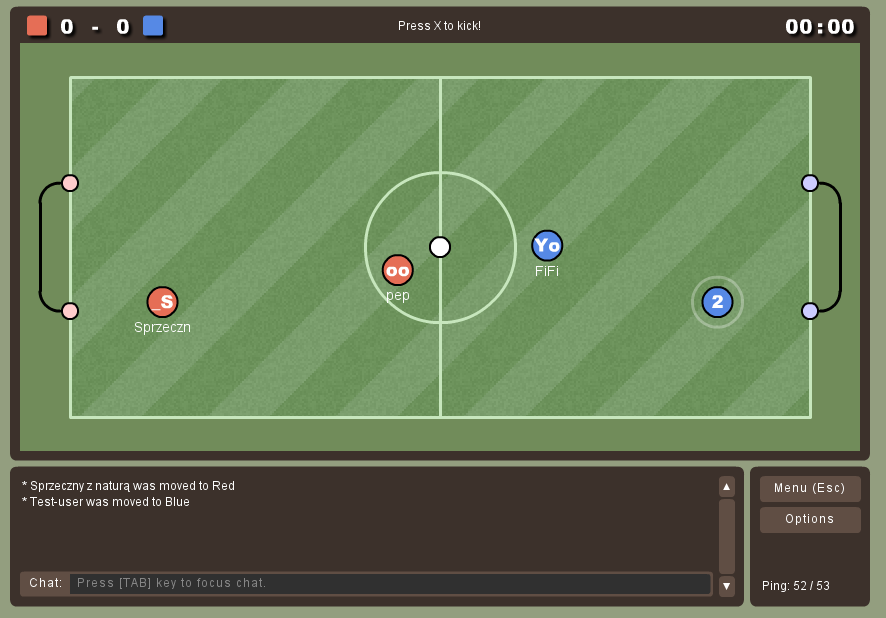
\includegraphics[width=0.9\textwidth]{imgs/haxball.png}
    \caption{Rozgrywka w HaxBall.}
    \label{fig:haxball}
\end{figure}

Tematem niniejszej pracy jest gra sieciowa, w której rozgrywka prowadzona jest w czasie rzeczywistym. W tym dokumencie zostaną przedstawione nie tylko szczegóły implementacji gry, lecz również, charakterysyka metodyki pracy zespołowej, która pozwoliła nam na szybką i owocną implementację projektu.

Gra, o której mowa, jest klonem internetowej gry HaxBall\footnote{\hyperref[http://www.haxball.com/]{http://www.haxball.com/}}. Jest to uproszczona wersja piłki nożnej, w której gracze wykorzystują tylko klawiaturę (strzałki oraz klawisz spacji aby dokonać kopnięcia w piłkę). Na rysunku \ref{fig:haxball} przedstawiono widok rozgrywki w grze.

W internecie dostępnych jest wiele gier tego typu, \emph{casual} bo o tym typie mowa, stał się bardzo ostatnimi czasy bardzo popularny (np. Angry Birds\footnote{\hyperref[http://chrome.angrybirds.com/]{http://chrome.angrybirds.com/}}). Jest to pierwszy z powodów, dla którego obraliśmy ten projekt. Drugim z powódów jest łatwość dekompozycji programu na niezależne (z punku wiedzenia pracy nad nimi) moduły, które mogą być osobno testowane, jednak na końcu dają się połączyć w jeden produkt. Łatwość dekopomozycji pozwala również na prosty przydział poszczególnych prac dla programistów.




